\clearpage
%===================================================================================
\section{ATLAS and CMS results included in the database update}
%===================================================================================


%-----------------------------------------------------------------------------------------------
\subsection{ATLAS Run~2 results for 36~fb$^{-1}$}
%-----------------------------------------------------------------------------------------------

The ATLAS Run~2 results included in this release are summarised in Table~\ref{tab:ATLASresults} and explained in more detail below.

\begin{table}[h]\centering
\begin{tabular}{l | ccccccc}
mode & $\gamma\gamma$ & $ZZ^*$ & $WW^*$ & $\tau\tau$ & $b\bar b$ & inv. \\
\hline
ggH & \cite{Aaboud:2018xdt} & \cite{Aaboud:2017vzb} & \cite{Aaboud:2018jqu} & \cite{Aaboud:2018pen} & -- & --\\
VBF &  \cite{Aaboud:2018xdt} & \cite{Aaboud:2017vzb} & \cite{Aaboud:2018jqu} & \cite{Aaboud:2018pen} & \cite{Aaboud:2018gay} & -- \\
WH & \multirow{2}{*}{\!\!\cite{Aaboud:2018xdt}} & \multirow{2}{*}{\!\!\cite{Aaboud:2017vzb}} & -- & -- & \cite{Aaboud:2017xsd} & -- \\
ZH &  &  & -- & -- & \cite{Aaboud:2017xsd} & \cite{Aaboud:2017bja} \\
ttH & \cite{Aaboud:2018xdt,Aaboud:2017jvq} & \cite{Aaboud:2017vzb,Aaboud:2017jvq} & \cite{Aaboud:2017jvq} & \cite{Aaboud:2017jvq} & \cite{Aaboud:2017jvq,Aaboud:2017rss} & -- \\ 
\end{tabular}
\caption{Overview of ATLAS Run~2 results included in this release.} 
\label{tab:ATLASresults}
\end{table}

%%% gamma gamma %%%

{\bf\boldmath $H\to\gamma\gamma$ (HIGG-2016-21):}  
The ATLAS analysis \cite{Aaboud:2018xdt} provides in Fig.~12 signal strengths for $H\to\gamma\gamma$ separated into   
ggH, VBF, VH and ``top'' (ttH+tH) production modes. No correlations are given for the signal strengths, but we can  
use instead the correlations for the stage-0 simplified template cross sections (STXS) provided in Fig.~40a of the ATLAS 
paper, which should be a close enough match. It turns out, however, that the $\mu$ values rounded to one decimal 
do not allow to reproduce very well the ATLAS coupling fits for $(C_V,\;C_F)$ or $(C_\gamma,\;C_g)$. 
We have therefore extracted the best-fit points and uncertainties 
from the 1D profile likelihoods, which are provided as Auxiliary Figures 23a--d on the analysis webpage, 
as %\footnote{In the XML file we use the exact numbers from the fit to the 1D profile likelihoods.}  
$\mu({\rm ggH},\,\gamma\gamma)\simeq 0.81^{+0.19}_{-0.18}$, 
$\mu({\rm VBF},\,\gamma\gamma)\simeq 2.04^{+0.61}_{-0.53}$, 
$\mu({\rm VH},\,\gamma\gamma)\simeq 0.66^{+0.89}_{-0.80}$ and 
$\mu({\rm ttH},\,\gamma\gamma)\simeq 0.54^{+0.64}_{-0.55}$ (using a Poisson likelihood).   
These numbers are consistent with the rounded values in Fig.~12 of \cite{Aaboud:2018xdt}, but using more digits 
improves the coupling fits as shown in Fig.~\ref{fig:validation_atlas_gamgam}.

\begin{figure}[h!]\centering
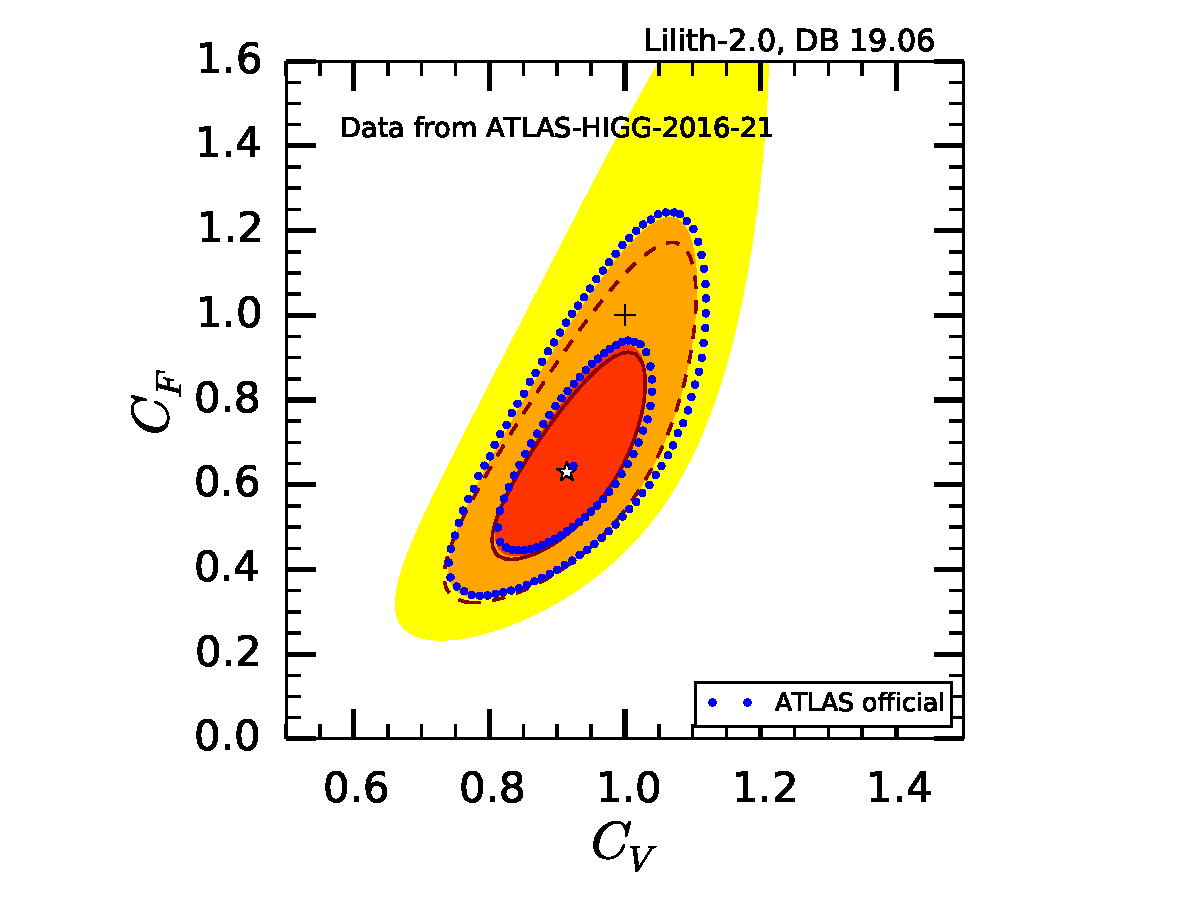
\includegraphics[width=0.55\textwidth]{validation/ATLAS/HIGG-2016-21-CVCF.pdf}%
\hspace{-16mm}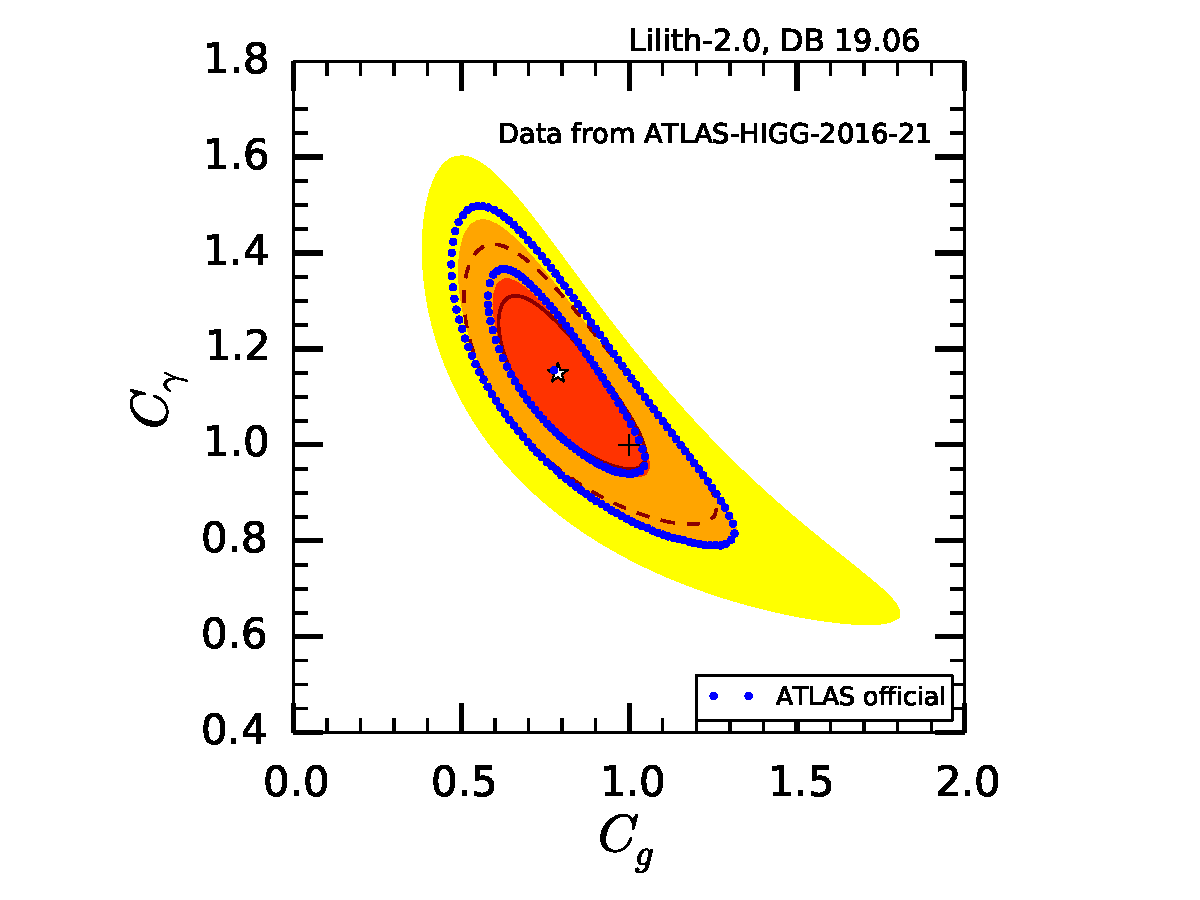
\includegraphics[width=0.55\textwidth]{validation/ATLAS/HIGG-2016-21-CgCGa.pdf}%
\vspace*{-2mm}
\caption{Fit of $C_F$ vs.\ $C_V$ (left) and $C_\gamma$ vs.\ $C_g$ (right) for data from the ATLAS $H\to\gamma\gamma$ analysis~\cite{Aaboud:2018xdt}. The red, orange and yellow filled areas show the 
$68\%$,  $95\%$ and $99.7\%$ CL regions obtained with {\tt Lilith} using best-fit values and uncertainties for the signal strengths 
as extracted from Aux.\ Figs.~23a--d of the ATLAS analysis together with the $4\times 4$ correlation matrix for the stage-0 STXS. 
This can be compared to the $68\%$,  $95\%$ CL contours obtained using the rounded values from Fig.~12 of \cite{Sirunyan:2018koj} 
(solid and dashed dark red lines) and to the official $68\%$ and $95\%$ CL contours from ATLAS (blue dots).}
\label{fig:validation_atlas_gamgam}
\end{figure}
 
%%% ZZ %%%

%{\bf\boldmath $H\to ZZ^*\to 4l$ (HIGG-2016-22):} A similar issue as discussed for $H\to\gamma\gamma$ above arises 
%for $H\to ZZ^*$, see the left panel in Fig.~\ref{fig:validation_atlas_ZZ}. Here we used the ggH and VBF signal strengths 
%given in Table~9 of \cite{Aaboud:2017vzb} with correlation $\rho=-0.41$ as of Aux.\ Fig.~4c, assuming a Poisson likelihood. 
%(This is a case were the variable Gaussian approximation performs less well). 
%For the VH and ttH production modes, lacking more information, we converted the given 95\%~CL limits into 
%$\mu({\rm VH},\,ZZ^*)=0^{+1.85}_{-0}$ and $\mu({\rm ttH},\,ZZ^*)=0^{+3.75}_{-0}$ using a 1-sided Gaussian. 
%The result is clearly not satisfactory. The closest match of the official CL contours is obtained if 
%we fit the 1D profile likelihoods for $\mu({\rm ggH},\,ZZ^*)$ and $\mu({\rm VBF},\,ZZ^*)$ shown in Aux.\ Figs.~7a and 7b 
%of \cite{Aaboud:2017vzb} as Poisson distributions. This gives $\mu({\rm ggH},\,ZZ^*)\simeq 1.12^{+0.25}_{-0.22}$ and 
%$\mu({\rm VBF},\,ZZ^*)\simeq 3.88^{+1.75}_{-1.46}$, which we implement as a bivariate Poisson distribution with    
%correlation $\rho=-0.41$ (from Aux.\ Fig.~4c of \cite{Aaboud:2017vzb}). The VH and ttH production modes are treated as before.
%As shown in the right panel of Fig.~\ref{fig:validation_atlas_ZZ}, this allows to reproduce reasonably well the $C_F$ vs.\ $C_V$ 
%fit from the ATLAS paper.

{\bf\boldmath $H\to ZZ^*\to 4l$ (HIGG-2016-22):} A similar issue as discussed for $H\to\gamma\gamma$ above arises 
for $H\to ZZ^*$. In order to reasonably reproduce the $C_F$ vs.\ $C_V$ fit of ATLAS (Fig.~8b of \cite{Aaboud:2017vzb}),  
we fit the 1D profile likelihoods for $\mu({\rm ggH},\,ZZ^*)$ and $\mu({\rm VBF},\,ZZ^*)$ shown in Aux.\ Figs.~7a and 7b 
of \cite{Aaboud:2017vzb} as Poisson distributions. This gives $\mu({\rm ggH},\,ZZ^*)\simeq 1.12^{+0.25}_{-0.22}$ and 
$\mu({\rm VBF},\,ZZ^*)\simeq 3.88^{+1.75}_{-1.46}$, which we implement as a bivariate Poisson distribution with    
correlation $\rho=-0.41$ (from Aux.\ Fig.~4c of \cite{Aaboud:2017vzb}). 
For the VH and ttH production modes, lacking more information, we convert the given 95\%~CL limits into 
$\mu({\rm VH},\,ZZ^*)=0\pm 1.89$ and $\mu({\rm ttH},\,ZZ^*)=0\pm 3.83$ using a 2-sided Gaussian 
(the same for 1-sided limits give a less good result when comparing to the ATLAS $C_F$ vs.\ $C_V$ fit). 
The validation is shown in Fig.~\ref{fig:validation_atlas_ZZ}. 
Note that this is a case where the variable Gaussian approximation performs less well that the Poisson likelihood. 

\begin{figure}[h!]\centering
%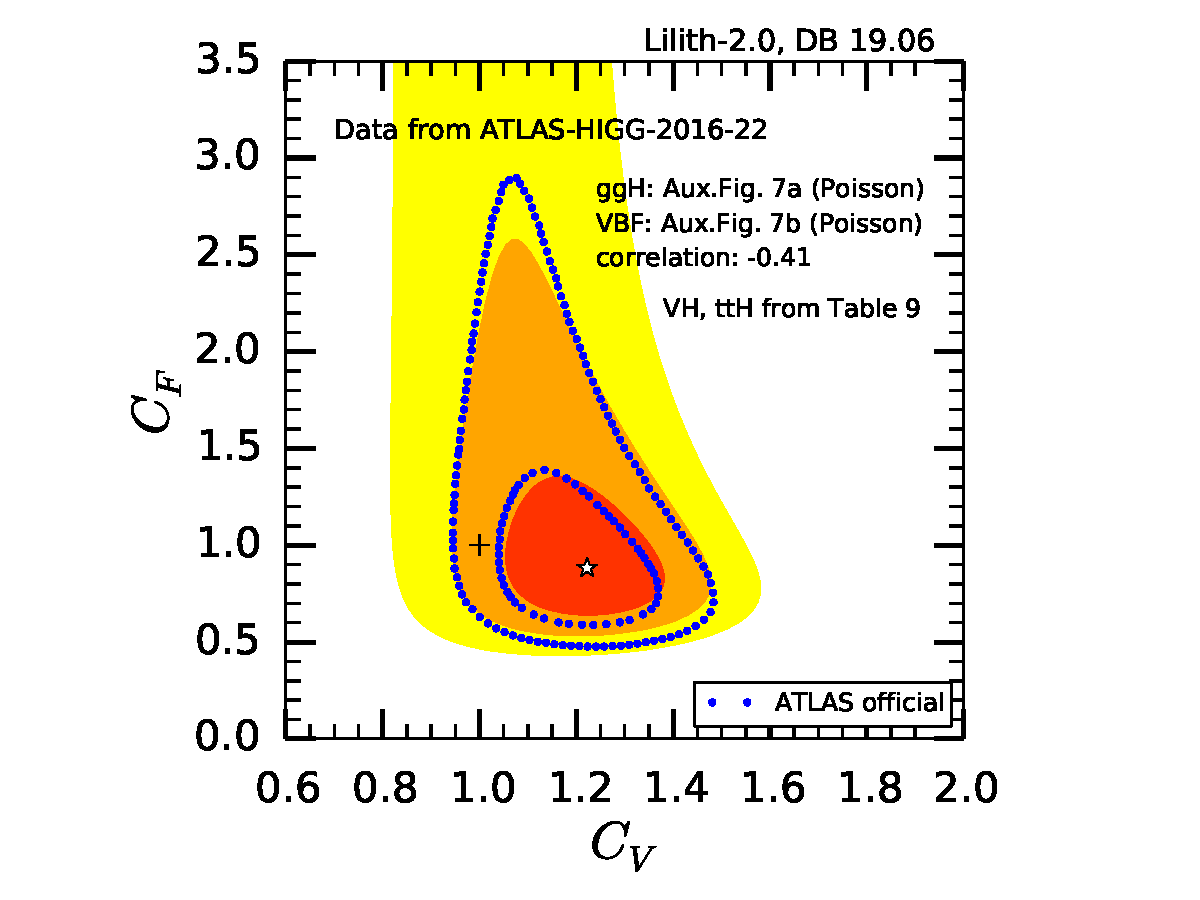
\includegraphics[width=0.54\textwidth]{validation/ATLAS/HIGG-2016-22-CVCF-fitted.pdf}%
\hspace{-12mm}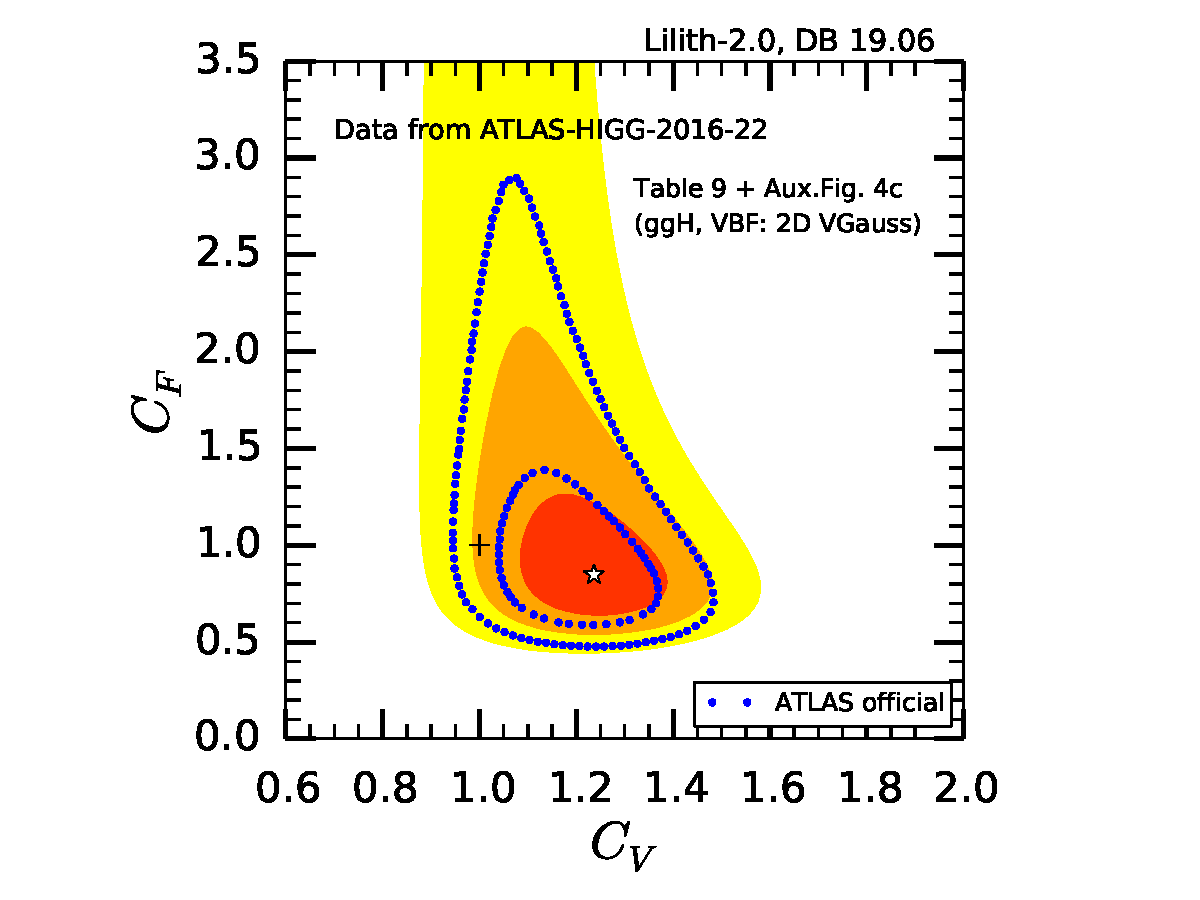
\includegraphics[width=0.41\textwidth]{validation/ATLAS/HIGG-2016-22-CVCF-official-vn.pdf}%
\hspace{-12mm}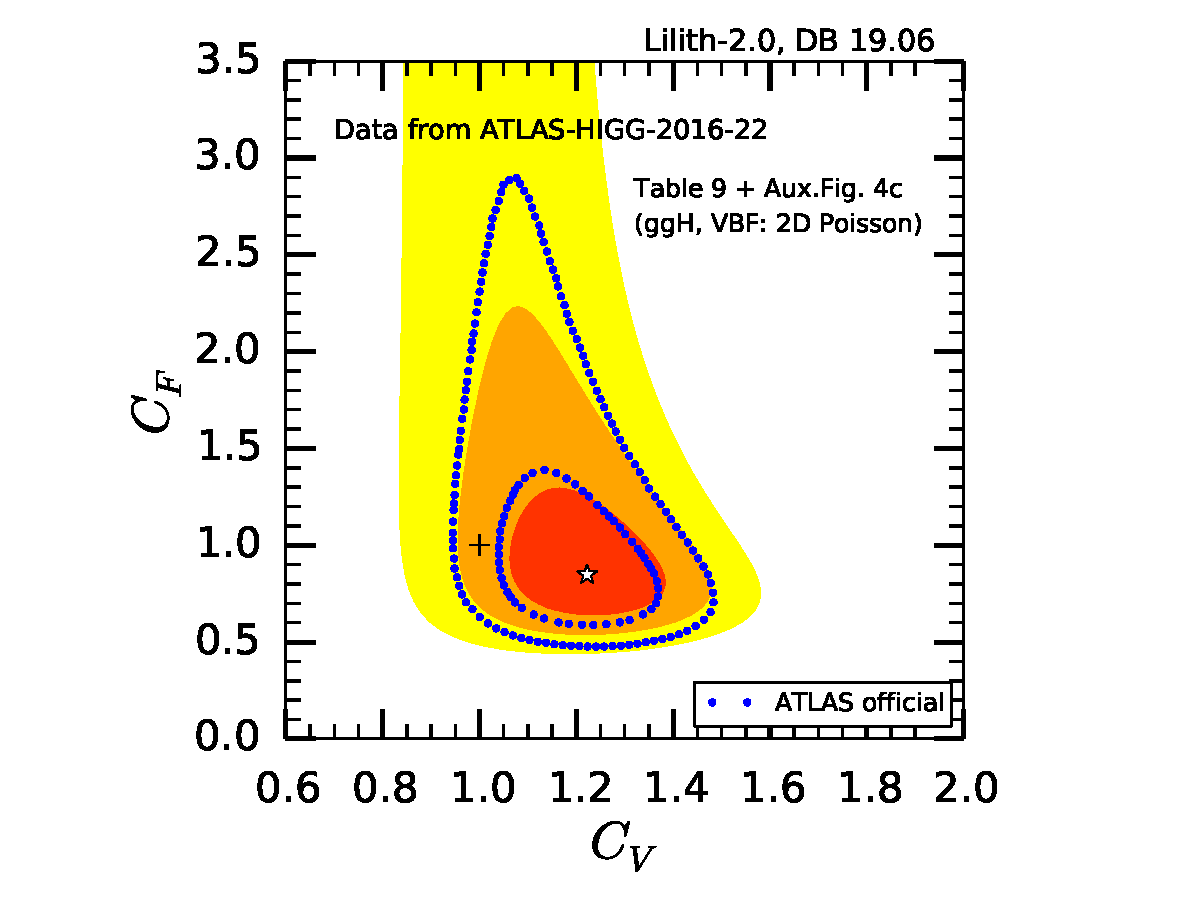
\includegraphics[width=0.41\textwidth]{validation/ATLAS/HIGG-2016-22-CVCF-official-p.pdf}%
\hspace{-12mm}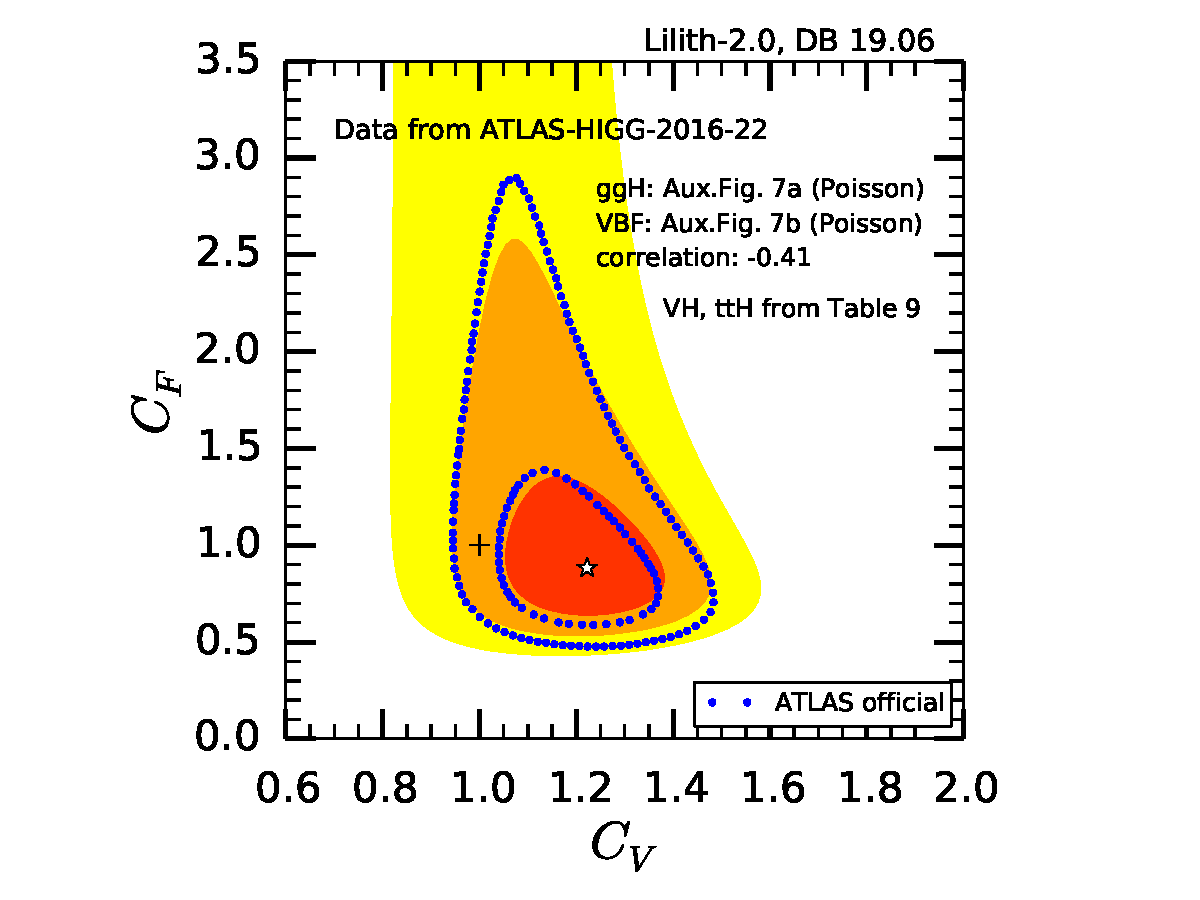
\includegraphics[width=0.41\textwidth]{validation/ATLAS/HIGG-2016-22-CVCF-fitted.pdf}\hspace{-12mm}%
\vspace*{-2mm}
\caption{Fit of $C_F$ vs.\ $C_V$ for data from the ATLAS $H\to ZZ^*$ analysis, 
%on the left using the values from Table~9 of~\cite{Aaboud:2017vzb}, on the right using 
using $\mu({\rm ggH},\,ZZ^*)$ and $\mu({\rm VBF},\,ZZ^*)$ as fitted from Aux.\ Figs.~7a and 7b of~\cite{Aaboud:2017vzb}; 
the ggH vs.\ VBF likelihood is then approximated as a bivariate Poissonian with correlation $-0.41$ (see text for more details). 
The $68\%$,  $95\%$ and $99.7\%$~CL regions obtained with {\tt Lilith} are shown as red, orange and yellow areas, 
and compared to the $68\%$ and  $95\%$~CL contours from ATLAS (in blue).}
\label{fig:validation_atlas_ZZ}
\end{figure}

%%% WW %%%

{\bf\boldmath $H\to WW^*\to 2l2\nu$ (HIGG-2016-07):} Ref.~\cite{Aaboud:2018jqu} focusses on the measurement of the 
inclusive ggH and VBF Higgs production cross sections in the $H\to WW^*\to e\nu\mu\nu$ channel. The paper quotes 
on page~13 signal strengths of $\mu({\rm ggH}, WW)=1.10^{+0.21}_{-0.20}$ and $\mu({\rm VBF}, WW)=0.62^{+0.36}_{-0.35}$. 
We implemented these as a 2D result with a correlation of $\rho=-0.08$ using the variable Gaussian approximation; 
the correlation was fitted from the $\sigma\times{\rm BR}$ plot, Fig.~9, of \cite{Aaboud:2018jqu}. 
%No coupling fits are available which could be used for validation. \\
As no other validation material is available, 
we show in Fig.~\ref{fig:validation_atlas_WW_tautau} (left) our reconstruction of the experimental likelihood in the 
$\mu({\rm ggH}, WW)$ vs.\ $\mu({\rm VBF}, WW)$ plane, comparing to the rescaled contours of Fig.~9 of the ATLAS paper.\\

%%% tau tau %%%

{\bf\boldmath $H\to \tau\tau$ (HIGG-2017-07):} This ATLAS cross section measurement in the $H\to \tau\tau$ channel~\cite{Aaboud:2018pen} 
provides as Aux.~Fig.~5 the 68\% and 95\% CL contours in the $\mu({\rm ggH}, \tau\tau)$ vs.\ $\mu({\rm VBF}, \tau\tau)$ plane. 
A fit of a bivariate variable Gaussian to the 95\%~CL contour in this plot  
gives $\mu({\rm ggH}, \tau\tau)\simeq 1.0^{+0.72}_{-0.59}$ and $\mu({\rm VBF}, WW)=1.20^{+0.62}_{-0.56}$ with 
$\rho = -0.45$, which are the values implemented in the database. 
As for $H\to WW$ above, no coupling fits are available which could be used for validation. 
We therefore show in Fig.~\ref{fig:validation_atlas_WW_tautau} (right) our reconstruction of the experimental likelihood in the 
$\mu({\rm ggH}, \tau\tau)$ vs.\ $\mu({\rm VBF}, \tau\tau)$ plane. 
Note that a fit to the 68\%~CL contour of ATLAS gives a less good result. \\

\begin{figure}[h!]\centering
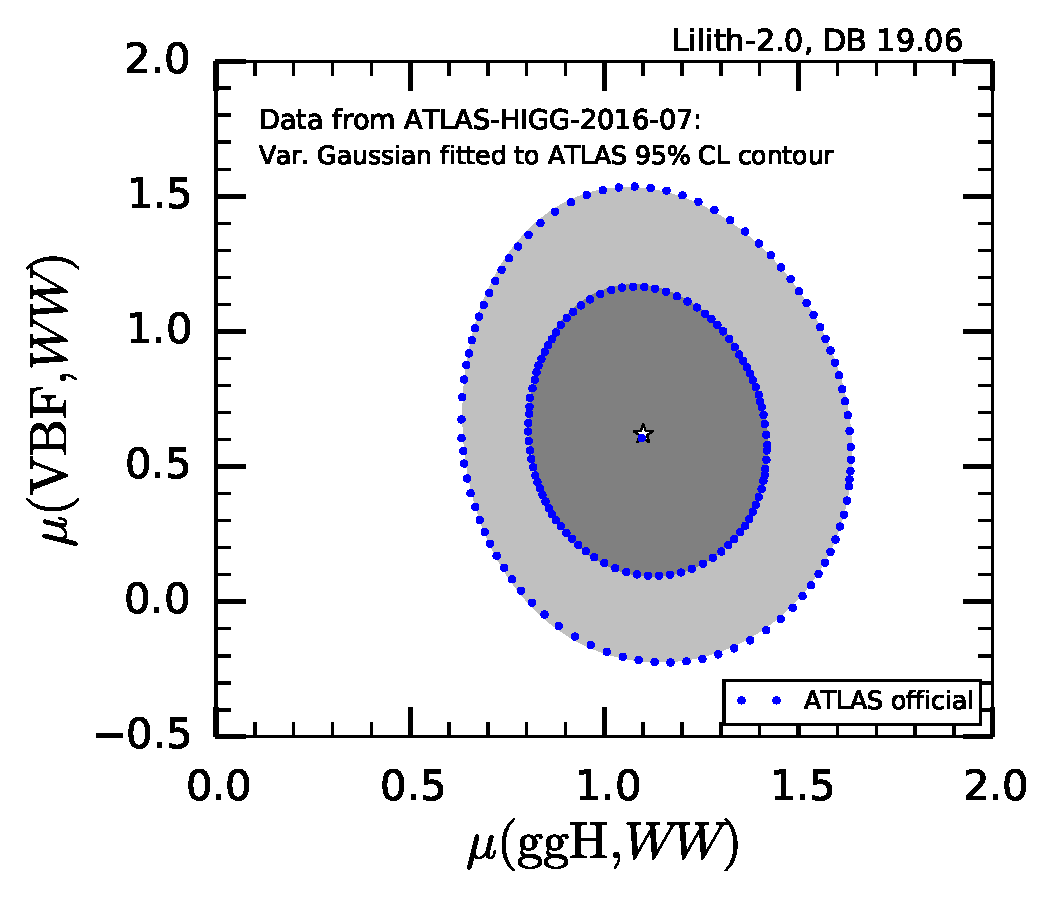
\includegraphics[width=0.46\textwidth]{validation/ATLAS/HIGG-2016-07-mu-2d.pdf}%
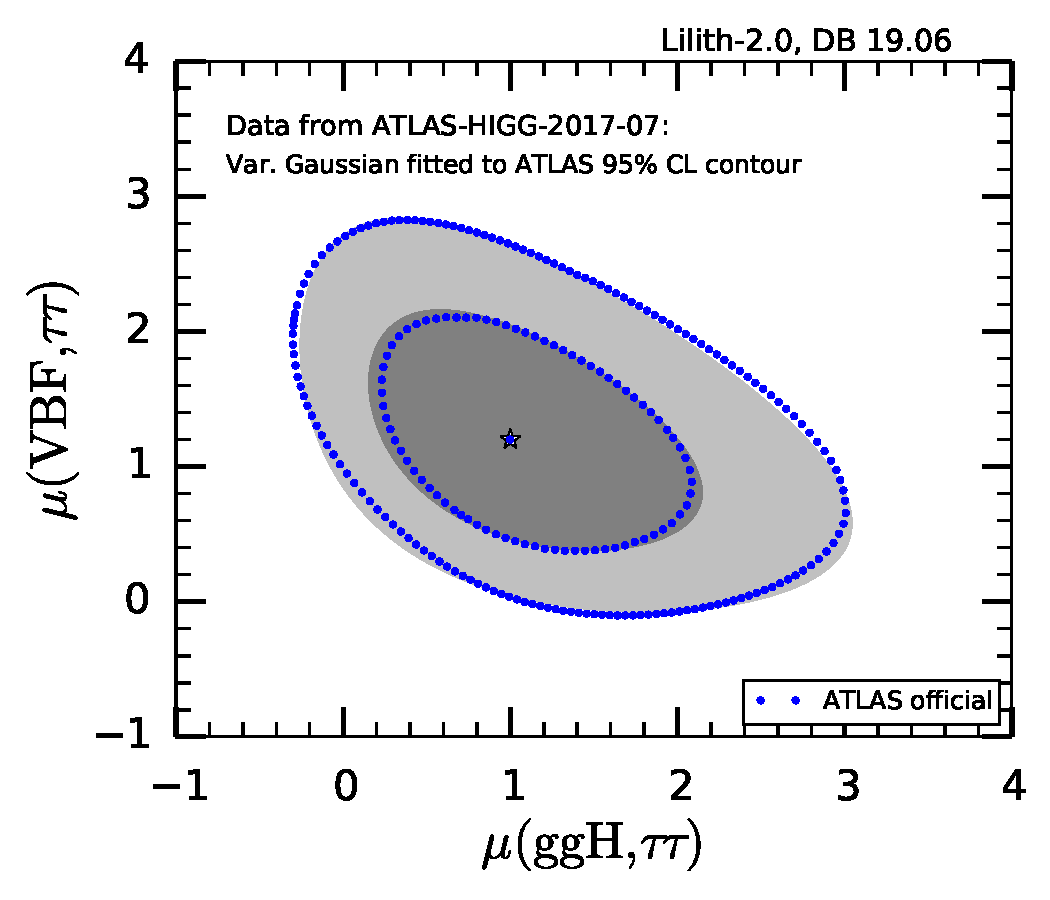
\includegraphics[width=0.46\textwidth]{validation/ATLAS/HIGG-2017-07-mu-2d.pdf}
\caption{Reconstruction of the experimental likelihood as 2D variable Gaussian %in the $\mu({\rm ggH}, \tau\tau)$ vs.\ $\mu({\rm VBF}, \tau\tau)$ plane. 
on the left for the $H\to WW$ channel from~\cite{Aaboud:2018jqu},
on the right for the $H\to \tau\tau$ channel from~\cite{Aaboud:2018pen}.  
The  $68\%$ and $95\%$~CL regions obtained with {\tt Lilith} are shown in dark and light gray, respectively, 
and compared to the $68\%$ and  $95\%$~CL contours from ATLAS (in blue).}
\label{fig:validation_atlas_WW_tautau}
\end{figure}

%%% b bbar %%%

{\bf\boldmath $H\to b\bar b$ (HIGG-2016-29 and HIGG-2016-30):} For the $H\to b\bar b$ decay mode, ATLAS gives 
$\mu({\rm ZH}, b\bar b) = 1.12^{+0.50}_{-0.45}$, $\mu({\rm WH}, b\bar b) = 1.35^{+0.68}_{-0.59}$~\cite{Aaboud:2018gay} 
and $\mu({\rm VBF}, b\bar b) = 3.0^{+1.7}_{-1.6}$~\cite{Aaboud:2018gay}. 
No correlation data is available, so we implemented each of these as a 1D result; 
a Poisson likelihood is assumed per default but can easily be changed to a variable Gaussian if the user wishes to do so. \\

%%% ttH %%%

{\bf\boldmath ttH production (HIGG-2017-02):} The ATLAS paper~\cite{Aaboud:2017jvq}, reporting evidence for $t\bar tH$ production,  
provides in Fig.~16 the signal strength results broken down into $H\to \gamma\gamma$, $VV~(=ZZ^*+WW^*)$, $\tau\tau$ and $b\bar b$ 
decay modes from a combined analysis of all $t\bar tH$ searches.  
Correlations are not given explicitly but can be estimated from %the 95\% CL contours of 
Figs.~17a and 17b in \cite{Aaboud:2017jvq} 
as $\rho(b\bar b, VV)\simeq 0.04$ for the correlation between the $H\to b\bar b$ and $H\to VV$ decay modes
and $\rho(\tau\tau, VV)\simeq -0.35$ for that between the $H\to \tau\tau$ and $H\to VV$ decay modes. 
In Fig.~\ref{fig:validation_atlas_ttH}, we compare the $C_F$ vs.\ $C_V$ fit from the implementation in {\tt Lilith} 
to the official one from~\cite{Aaboud:2017jvq}. 
%While the agreement is not very good,  
%one has to note that without the correlations quoted above the situation is much worse. 

\begin{figure}[htb!]\centering
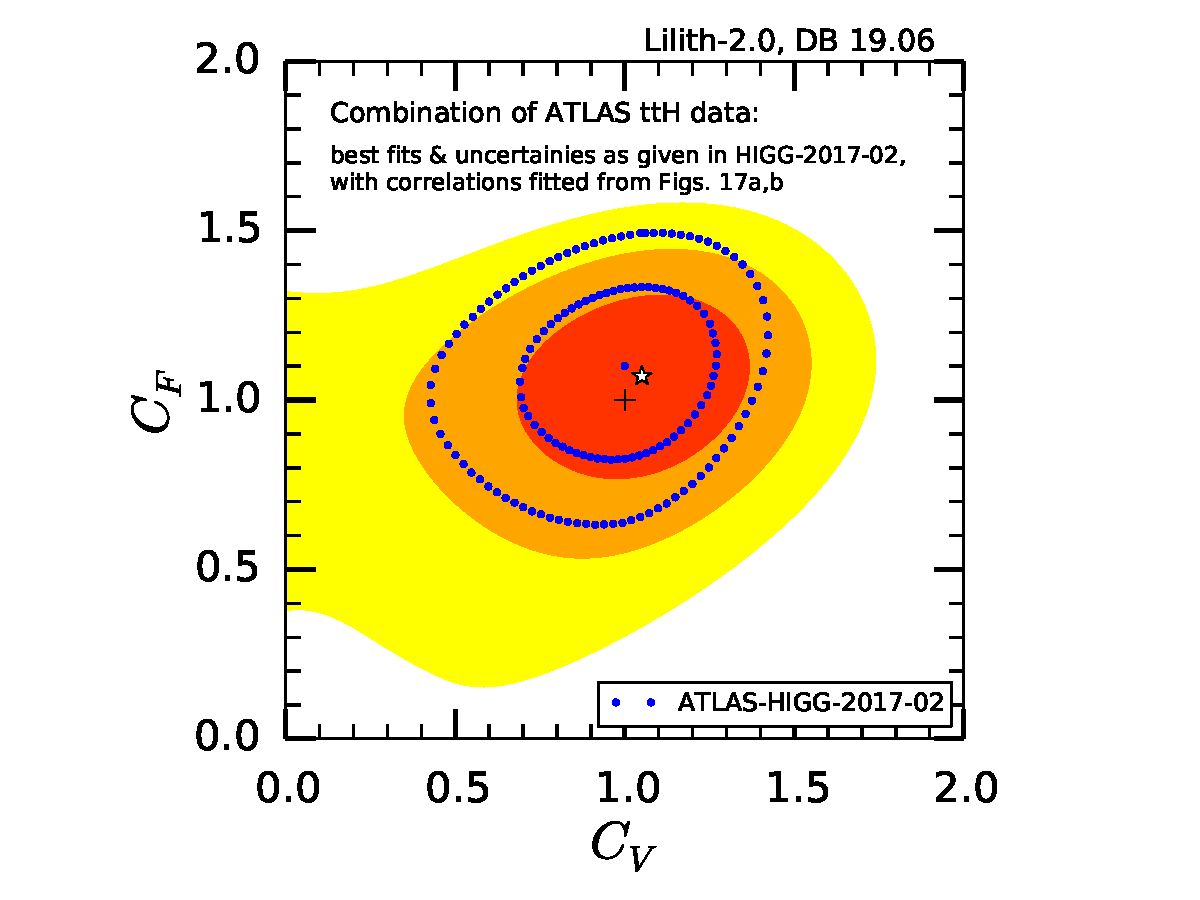
\includegraphics[width=0.55\textwidth]{validation/ATLAS/HIGG-2017-02-CVCF-off-corr.pdf}% 
\hspace{-16mm}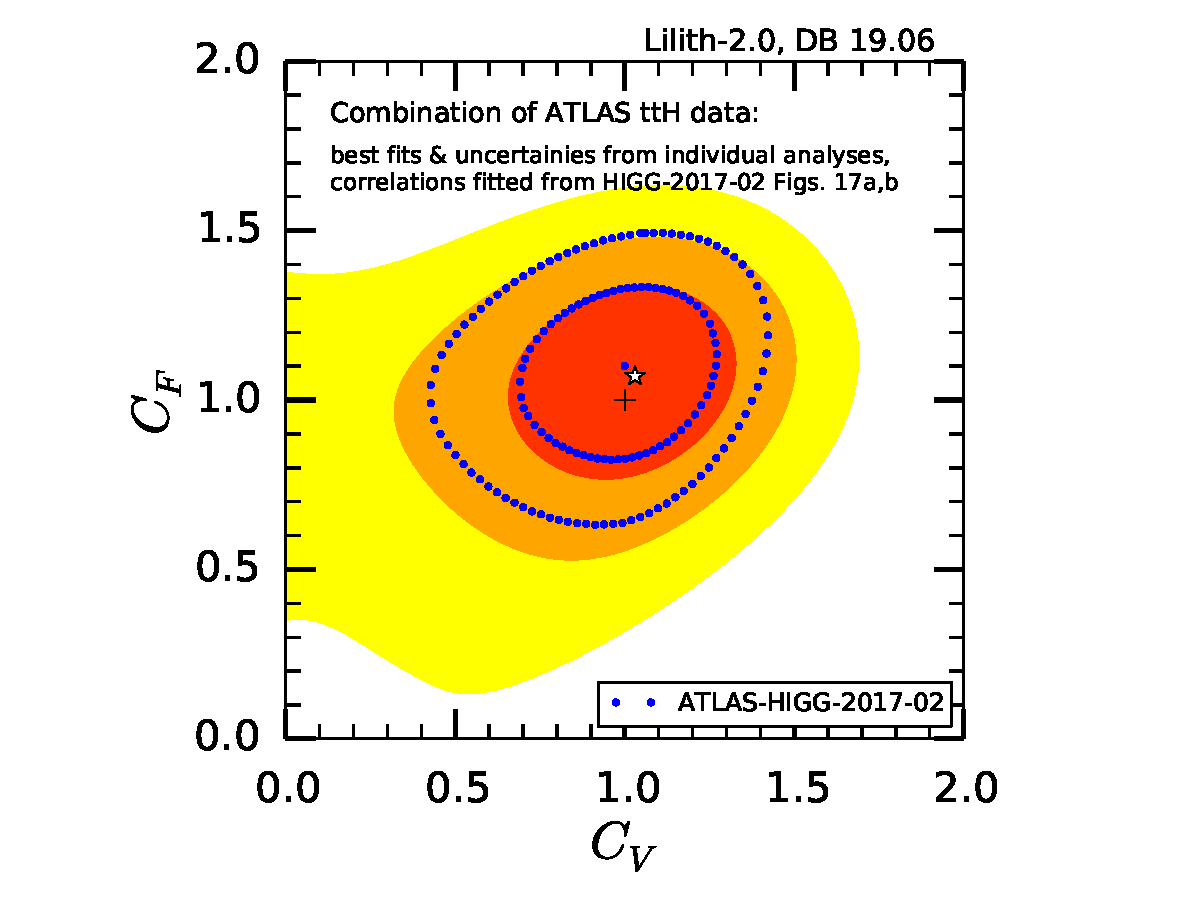
\includegraphics[width=0.55\textwidth]{validation/ATLAS/HIGG-2017-02-CVCF-fit-corr.pdf}%
\vspace*{-2mm}
\caption{Fit of $C_F$ vs.\ $C_V$ from a combination of the ATLAS ttH measurements, ....
%on the left without and on the right with the 
%correlations fitted from Figs.~17a,b in \cite{Aaboud:2017jvq} (see text for details). 
The  $68\%$,  $95\%$ and $99.7\%$~CL regions obtained with {\tt Lilith} are shown as red, orange and yellow areas, 
and compared to the $68\%$,  $95\%$~CL contours from ATLAS (in blue).}
\label{fig:validation_atlas_ttH}
\end{figure}

A few comments are in order here. First, the measurement of $\mu({\rm t\bar tH},\,\gamma\gamma)$ actually comes from 
\cite{Aaboud:2018xdt} (HIGG-2016-21, see above) and is also included in the HIGG-2016-21 XML file; 
to avoid overlap when using both the HIGG-2016-21 and HIGG-2017-02 datasets, we provide a 3D XML file for the latter 
which includes only the $VV$, $\tau\tau$ and $b\bar b$, but not the $\gamma\gamma$, decay modes. 
Second, the individual measurement \cite{Aaboud:2017rss} gives $\mu({\rm t\bar tH},\,b\bar b)$ to two decimals 
($0.84^{+0.64}_{-0.61}$) instead just one ($0.8\pm 0.6$) in \cite{Aaboud:2017jvq}. Since this makes a visible difference 
in Fig.~\ref{fig:validation_atlas_ttH}, improving the quality of the fit, we use the more precise numbers from  \cite{Aaboud:2017rss}. 
Third, for $\mu({\rm t\bar tH},\,VV)$ the contribution from $H\to WW^*$ should dominate, but the concrete weights of the 
$ZZ^*$ and $WW^*$ decay modes are not given in~\cite{Aaboud:2017jvq}. This is not a problem as long as $C_Z=C_W\equiv C_V$, but one should 
not use the HIGG-2017-02 XML file for any other case.\\

{\bf\boldmath $H\to$~invisible (HIGG-2016-28):} 
Results from the search for invisibly decaying Higgs bosons produced in association with a $Z$ boson are presented in \cite{Aaboud:2017bja}. 
A 95\%~CL upper limit of BR$(H\to {\rm inv.})<0.67$ is set for $m_H= 125$~GeV assuming the SM $ZH$ production cross section. 
In the {\tt Lilith} database, 
we use a likelihood grid as function BR$(H\to {\rm inv.})$ extracted from Aux. Fig.~1c on the analysis' webpage. \\



%\clearpage
%-----------------------------------------------------------------------------------------------
\subsection{CMS Run~2 results for 36~fb$^{-1}$}
%-----------------------------------------------------------------------------------------------

The CMS Run~2 results included in this release are summarised in Table~\ref{tab:CMSresults} and explained in more detail below.

\begin{table}[h]\centering
\begin{tabular}{l | ccccccc}
mode & $\gamma\gamma$ & $ZZ^*$ & $WW^*$ & $\tau\tau$ & $b\bar b$ & $\mu\mu$ & inv. \\
\hline
ggH & \cite{Sirunyan:2018koj} & \cite{Sirunyan:2018koj} & \cite{Sirunyan:2018koj} & \cite{Sirunyan:2018koj} & \cite{Sirunyan:2018koj} & \cite{Sirunyan:2018koj} & \cite{Sirunyan:2018owy} \\
VBF &  \cite{Sirunyan:2018koj} & \cite{Sirunyan:2018koj} & \cite{Sirunyan:2018koj} & \cite{Sirunyan:2018koj} &-- & \cite{Sirunyan:2018koj} & \cite{Sirunyan:2018owy} \\
WH &  \cite{Sirunyan:2018koj} & \cite{Sirunyan:2018koj} & \cite{Sirunyan:2018koj} & \cite{Sirunyan:2018cpi} & \cite{Sirunyan:2018koj} & -- & \cite{Sirunyan:2018owy} \\
ZH & \cite{Sirunyan:2018koj} & \cite{Sirunyan:2018koj} & \cite{Sirunyan:2018koj} & \cite{Sirunyan:2018cpi} & \cite{Sirunyan:2018koj} & -- & \cite{Sirunyan:2018owy} \\
ttH & \cite{Sirunyan:2018koj} & \cite{Sirunyan:2018koj} & \cite{Sirunyan:2018koj} & \cite{Sirunyan:2018koj} & \cite{Sirunyan:2018koj} & -- & -- \\
\end{tabular}
\caption{Overview of CMS Run~2 results included in this release. Note that we use the full $24\times 24$ correlation matrix 
for the signal strengths for each production and decay mode combination provided in \cite{Sirunyan:2018koj}.}
\label{tab:CMSresults}
\end{table}


{\bf\boldmath Combined measurements (HIG-17-031):} 
CMS presented in \cite{Sirunyan:2018koj} a combination of the individual measurements for the 
$H\to \gamma\gamma$~\cite{Sirunyan:2018ouh}, $ZZ$~\cite{Sirunyan:2017exp}, $WW$~\cite{Sirunyan:2018egh}, 
$\tau\tau$~\cite{Sirunyan:2017khh}, $b\bar b$~\cite{Sirunyan:2017elk,Sirunyan:2017dgc} and $\mu\mu$~\cite{Sirunyan:2018hbu} 
decay modes as well as the $t\bar tH$ analyses~\cite{Sirunyan:2018shy,Sirunyan:2018mvw,Sirunyan:2018ygk}. 
We use the best fit values and uncertainties for the signal strengths for each production %(ggH, VBF, WH, ZH, ttH) 
and decay  %($\gamma\gamma$, $ZZ$, $WW$, $\tau\tau$, $b\bar b$, $\mu\mu$) 
mode combination presented in Table~3 of \cite{Sirunyan:2018koj} together with the $24\times 24$ correlation matrix 
provided as ``Additional Figure~1'' on the analysis webpage. As shown in Figs.~\ref{fig:validation_cms_combination} 
and \ref{fig:validation_cms_2hdm}, 
this allows to reproduce well the coupling fits of the CMS paper.\\

\begin{figure}[hbt!]\centering
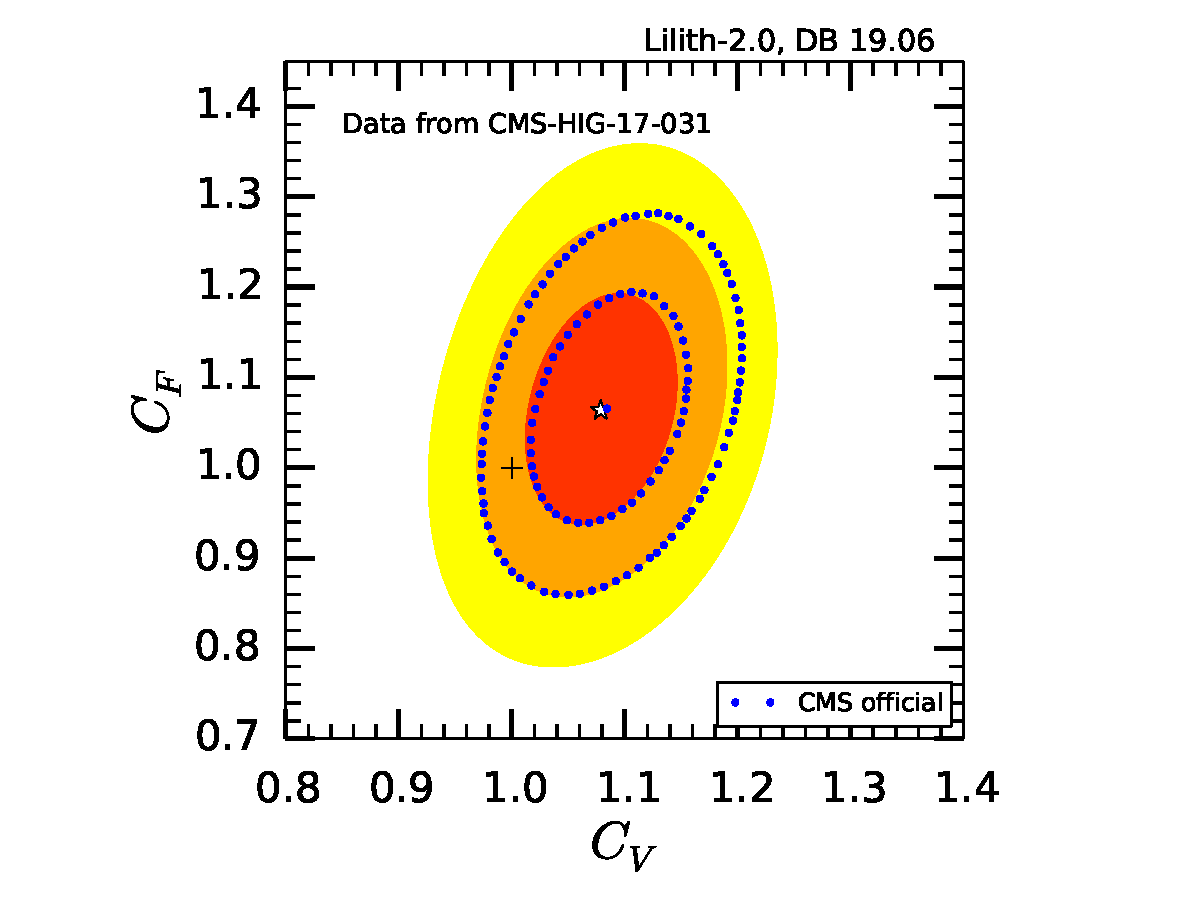
\includegraphics[width=0.65\textwidth]{validation/CMS/HIG-17-031-CVCF.pdf}%
\vspace*{-2mm}
\caption{Fit of $C_F$ vs.\ $C_V$ using best-fit values and uncertainties for the signal strengths for each production (ggH, VBF, WH, ZH, ttH) 
and decay ($\gamma\gamma$, $ZZ$, $WW$, $\tau\tau$, $b\bar b$, $\mu\mu$) mode combination together with the 
$24\times 24$ correlation matrix from the CMS combination paper~\cite{Sirunyan:2018koj}. 
The  $1\sigma$,  $2\sigma$ and $3\sigma$ regions obtained with {\tt Lilith} are shown as red, orange and yellow areas, 
and compared to the $1\sigma$ and $2\sigma$ contours from CMS (blue dots).}
\label{fig:validation_cms_combination}
\end{figure}

\begin{figure}[t!]\centering
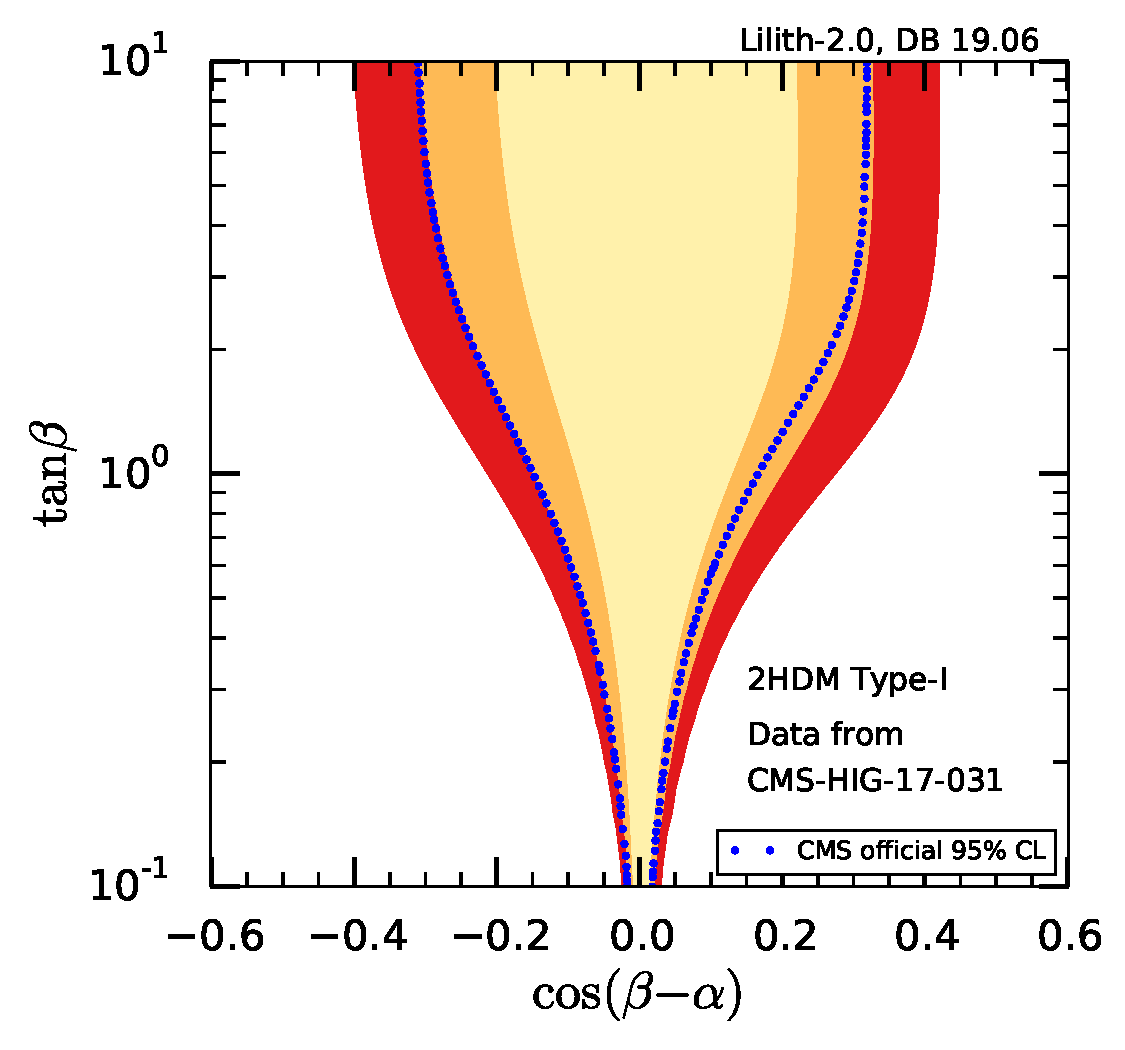
\includegraphics[width=0.5\textwidth]{validation/CMS/HIG-17-031-2HDM-Type1.pdf}%
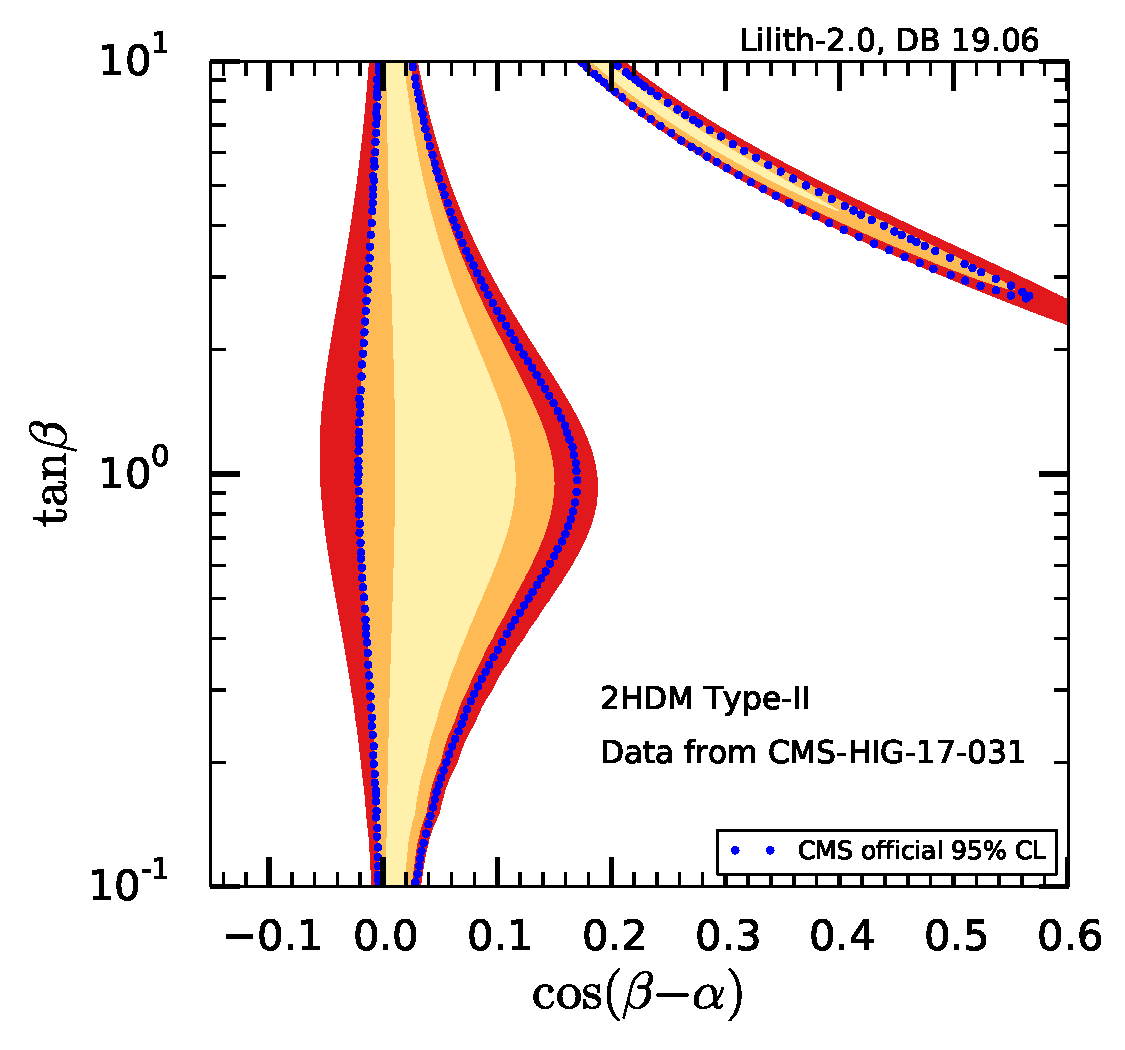
\includegraphics[width=0.5\textwidth]{validation/CMS/HIG-17-031-2HDM-Type2.pdf}%
\vspace*{-2mm}
\caption{Fit of $\tan\beta$ vs.\ $\cos(\beta-\alpha)$ for the Two-Higgs-Doublet models of Type~I (left) and Type~II (right) 
using the data from the combined CMS measurement~\cite{Sirunyan:2018koj}. 
The beige, orange and red filled areas show the 68\%, 95\% and 99.7\% CL regions obtained with {\tt Lilith}, 
while the blue dots mark the 95\% CL contours from CMS.}
\label{fig:validation_cms_2hdm}
\end{figure}

{\bf\boldmath $VH$, $H\to\tau\tau$ (HIG-18-007)}: The above data from \cite{Sirunyan:2018koj} is supplemented by the results 
for the $\tau\tau$ decay mode from the $WH$ and $ZH$ targeted analysis \cite{Sirunyan:2018cpi}. These are implemented in the 
form of 1D intervals for $\mu(ZH,\;H\to\tau\tau)$ and $\mu(WH,\;H\to\tau\tau)$ taken from Fig.~6 of \cite{Sirunyan:2018cpi}. \\

{\bf\boldmath $H\to$~invisible (HIG-17-023)}: 
In \cite{Sirunyan:2018owy}, CMS performed a search for invisible decays of a Higgs boson produced through vector boson fusion. 
We use the profile likelihood ratios for the qqH-tag, Z(ll)H-, V(qq')H- and ggH-tag categories extracted 
from their Fig.~8b together with the relative contributions from the different Higgs production mechanisms  
given in Table~6 of that paper. This assumes that the relative signal contributions stay roughly the same as for 
SM production cross sections. For validation, we reproduce in Fig.~\ref{fig:validation_cms_inv}
 the $C_g$ vs.\ $C_\gamma$ fit of \cite{Sirunyan:2018koj}, where the branching ratios of invisible and undetected decays 
are treated as free parameters.%%
\footnote{The profiling in Fig.~\ref{fig:validation_cms_inv} was done with {\tt Minuit}. 
  Since {\tt Minuit} does not allow conditional limits, in this case ${\rm BR}(H\to {\rm inv.})+{\rm BR}(H\to {\rm undetected})<1$, 
  we demanded that both BR$(H\to {\rm inv.})$ and BR$(H\to {\rm undetected})$ be less than 50\%.} 

\begin{figure}[h!]\centering
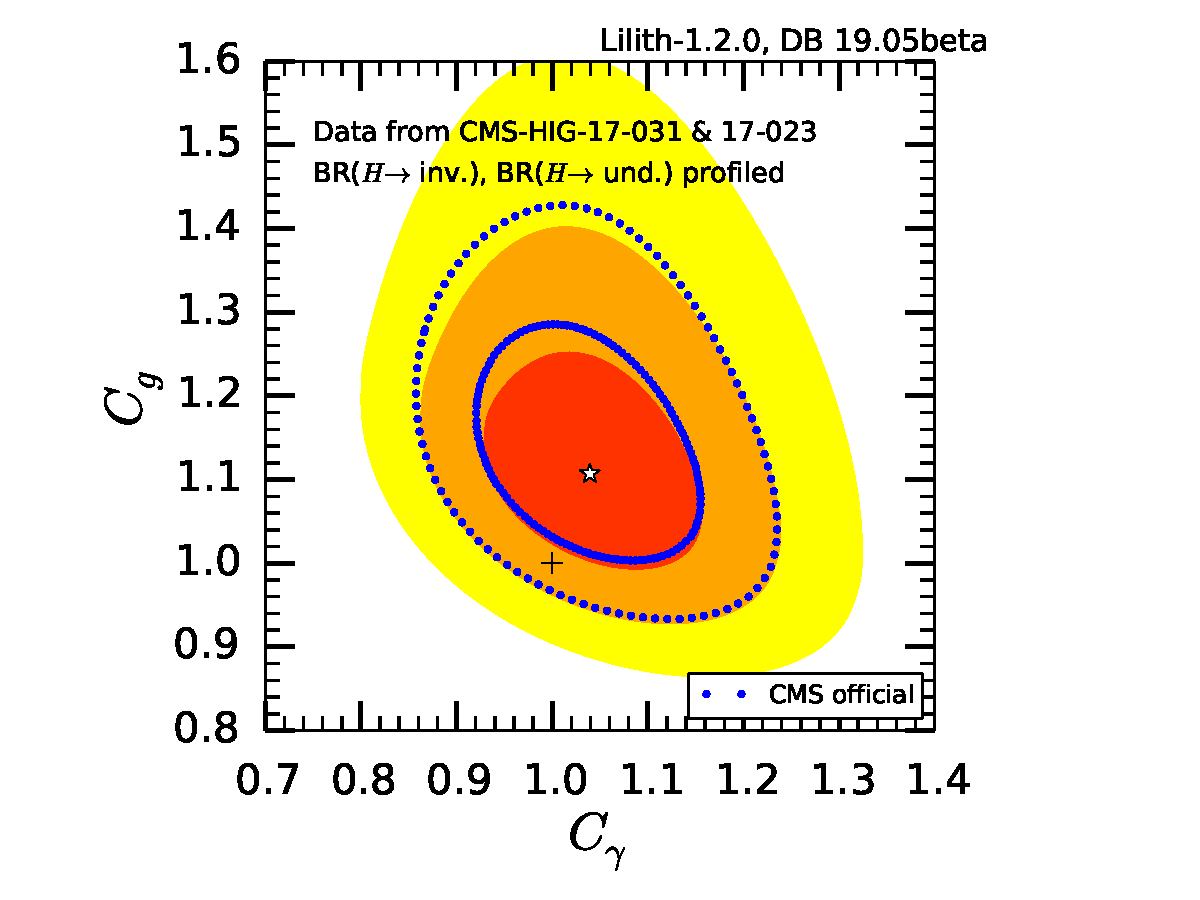
\includegraphics[width=0.65\textwidth]{validation/CMS/HIG-17-031-CgCGa_BRinvBRund_profiled.pdf}%
\vspace*{-2mm}
\caption{Fit of $C_g$ vs.\ $C_\gamma$ using the data from the combined CMS measurement~\cite{Sirunyan:2018koj} and the 
search for invisible decays of a Higgs boson~\cite{Sirunyan:2018owy}. The branching ratios of invisible and undetected decays 
are treated as free parameters in the fit. 
The  $1\sigma$,  $2\sigma$ and $3\sigma$ regions obtained with {\tt Lilith} are shown as red, orange and yellow areas, 
and compared to the $1\sigma$ and $2\sigma$ contours from CMS (in blue).}
\label{fig:validation_cms_inv}
\end{figure}

